\documentclass{../../kalkulus-ppt}



\author[Tetew]{Teosofi Hidayah Agung}
\date{19 September 2024}
\title[Kalkulus 1 - Bab 5]{Aplikasi Turunan}
\institute[Matematika ITS]{Departemen Matematika\\ Institut Teknologi Sepuluh Nopember}
\titlegraphic{{
\includegraphics[scale=0.3]{ITS.png}$\quad$
\includegraphics[scale=0.02]{M.png}}}

\newcommand{\dom}{\mathcal{D}}
\newcommand{\rng}{\mathcal{R}}

\renewcommand{\arraystretch}{1.5}

\begin{document}
{\usebackgroundtemplate{
  \tikz[overlay,remember picture] \node[opacity=0.09, at=(current page.center)]{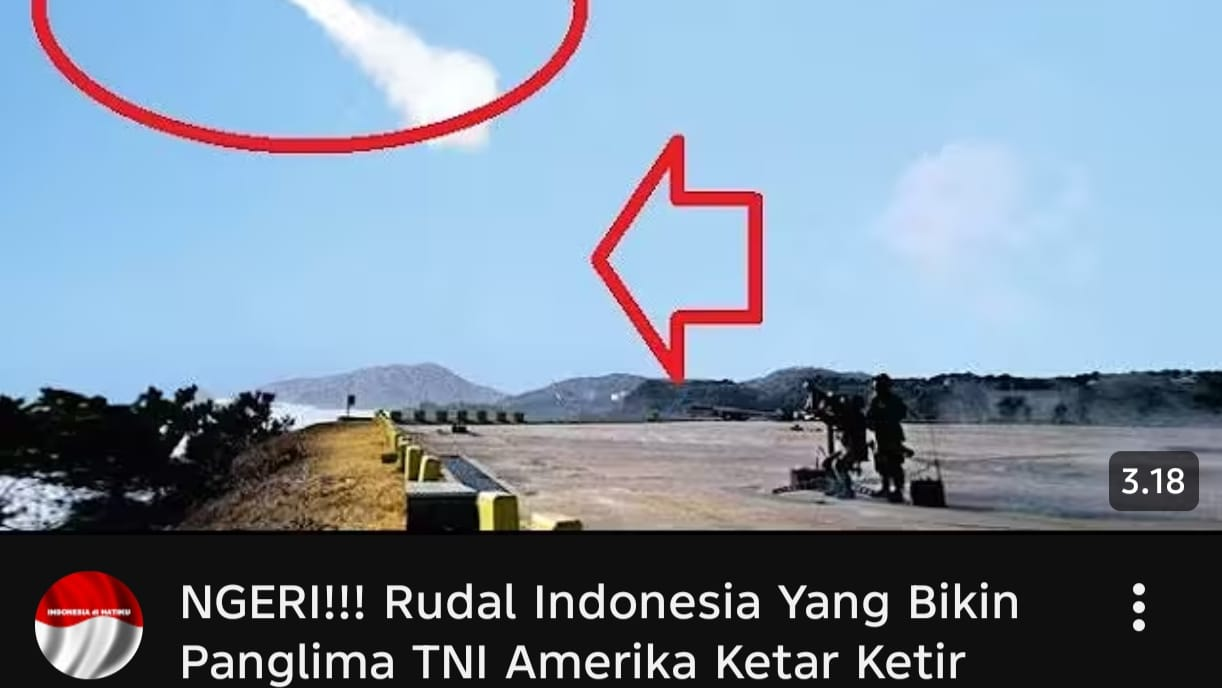
\includegraphics[width=\paperwidth]{TNIamerika.png}};}
\begin{frame}
  \titlepage
\end{frame}
}

\AtBeginSection{
  {
      \begin{frame}{Daftar isi}
        \tableofcontents[currentsection]
        % \begin{tikzpicture}[overlay, remember picture] 
        %     \node at ([yshift=.5cm]current page.south east) [
        %         anchor = south east, 
        %         ] {
        %     \animategraphics[autoplay,loop,width=0.2\textwidth]{30}{Arisu Dance/Arisu Dance-}{0}{186}
        %     };
        % \end{tikzpicture}
      \end{frame}}
}

\section{Laju-laju yang Berkaitan}
\begin{frame}

\end{frame}

\end{document}